\chapter{Objetivos}
\label{cap:capitulo2}

En esta sección del documento se describe el problema a resolver, marcando los objetivos y requisitos pautados en el desarrollo de este \ac{TFG}.

\section{Descripción del problema}
\label{sec:descripcion}

El objetivo principal de este \ac{TFG} es desarrollar un primer paso para un sistema de conducción autónoma capaz de desenvolverse eficientemente en entornos urbanos. Para lograrlo, se emplean técnicas de \ac{DRL} para la toma de decisiones, junto con diferentes enfoques de \ac{DL} para la percepción del entorno, con el objetivo de garantizar un comportamiento robusto, seguro y eficiente. El proyecto se centra en conseguir una conducción segura y estable durante todo el recorrido, abordando tres tareas principales: seguimiento del carril, control de crucero adaptivo y llevar a cabo una maniobra de adelantamiento completa.

A continuación, se definen los siguientes sub-objetivos: 

\begin{enumerate}
\item Implementación de un módulo de percepción basado en el \ac{LiDAR}, para identificar obstáculos en la carretera, y en cámaras RGB que, combinadas con técnicas de \ac{DL} para el post-procesado, permiten segmentar de la calzada y detectar del carril.
\item Desarrollo de un comportamiento de sigue-carril.
\item Ampliación del comportamiento sigue-carril para incorporar un control de crucero adaptativo, el cual se centra en ajustar la velocidad del coche autónomo a la del vehículo que circula delante.
\item Desarrollo de un modelo capaz de ejecutar maniobras completas de adelantamiento, incluyendo el cambio de carril y la vuelta al mismo.
\item Análisis y comparación de los diferentes comportamientos de conducción autónomos desarrollados.
\end{enumerate}

\section{Requisitos}
\label{sec:requisitos}

Los requisitos que han de cumplirse en este trabajo son:
\begin{enumerate}
\item Uso del entorno de simulación CARLA\footnote{\url{https://carla.org/}}, el cual permite la simulación de escenarios realistas, diversos comportamientos de vehículos y la prueba de modelos. Al ser un simulador ampliamente reconocido en el ámbito de la conducción autónoma, garantiza la reutilización del proyecto en aplicaciones futuras de este campo.
\item Usar modelos de \ac{DL} para la percepción visual y algoritmos de \ac{DRL} para la toma de decisiones.
\item Lograr un comportamiento sigue-carril estable y sin oscilaciones, alcanzando velocidades en torno a los 70 km/h.
\item Mantener un control de crucero adaptativo respecto al vehículo delantero, asegurando una distancia de seguridad adecuada conforme a las normas de la \ac{DGT}\footnote{\url{https://www.dgt.es/export/sites/web-DGT/.galleries/downloads/conoce-el-estado-del-trafico/operaciones-especiales/4_O.-E.-Primero-de-Mayo-2023_Consejos-y-normas-de-Seguridad-Vial_V-I.pdf}}.
\item Llevar a cabo un adelantamiento seguro en todo momento, comprobando si existe un carril al que podamos desplazarnos y asegurando que la maniobra de retorno al carril inicial no pone en peligro al otro agente en la vía.
\end{enumerate}

\section{Metodología}
\label{sec:metodologia}

Este TFG comenzó en febrero de 2024 y finalizó en marzo de 2025. La metodología de trabajo fue la siguiente:

\begin{itemize}
\item Se ha utilizado la metodología \textit{Scrum}\footnote{\url{https://www.nimblework.com/agile/scrum-methodology/}}, la cual consiste en organizar el trabajo en ciclos cortos llamados \textit{sprints}, que suelen durar entre una y cuatro semanas. Esta metodología fomenta una organización eficiente al dividir el trabajo en tareas pequeñas y manejables, promoviendo la iteración y mejora continua al revisar y ajustar el trabajo regularmente.
\item Durante cada \textit{sprint}, se realizaron reuniones semanales a través de \textit{Teams}\footnote{\url{https://www.microsoft.com/es-es/microsoft-teams/log-in}}, con una duración de 30-60 minutos, para hacer un seguimiento de los problemas que hubieran podido surgir a lo largo de la semana y definir los nuevos objetivos a cumplir.
\item Contacto mediante el email de la universidad con el fin de resolver problemas urgentes e intercambiar contenido de avances significativos.
\item Se utilizó un repositorio de \textit{GitHub}\footnote{\url{https://github.com/RoboticsLabURJC/2024-tfg-lara-poves/}} para gestionar el control de versiones del código fuente, los modelos y los datos más relevantes generados durante el desarrollo del proyecto. En la Figura \ref{fig:github}, se observa que la mayor carga de trabajo tuvo lugar al inicio, coincidiendo con la creación de los entornos de desarrollo y la implementación del módulo de percepción. Posteriormente, se llevaron a cabo los entrenamientos y pruebas de los modelos, ajustando los hiperparámetros de entrenamiento e intentando mejorar los resultados obtenidos. Finalmente, se ve un último \textit{sprint} referente a la elaboración de la memoria y a los ajustes finales en los entrenamientos del adelantamiento.

\begin{figure}[ht]
\centering
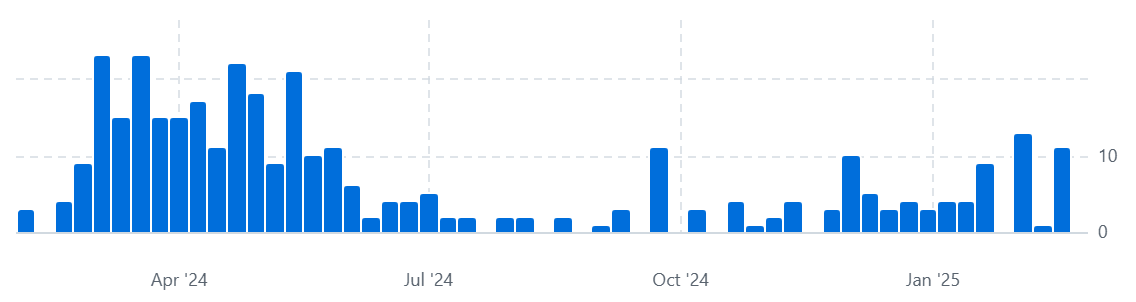
\includegraphics[width=9cm]{figs/objetivos/github.png}
\caption{Seguimiento de trabajo en GitHub.}
\label{fig:github}
\end{figure}

\item Mantenimiento de un \textit{blog}\footnote{\url{https://roboticslaburjc.github.io/2024-tfg-lara-poves/}} para documentar problemas, avances e investigaciones realizadas durante el desarrollo del proyecto, asegurando un registro del progreso y soluciones a los desafíos plateados.

\end{itemize}

\section{Plan de trabajo}
\label{sec:plantrabajo}

Finalmente, los pasos a seguir fueron:

\begin{enumerate}
\item Comienzo del trabajo:
\begin{itemize}
\item Desde el inicio, el tema del proyecto estuvo claro, centrado en la conducción autónoma en el simulador CARLA y algoritmos basados en \ac{DRL}.
\item Se gestionó el acceso al servidor donde se desarrollaría el proyecto, el cual ya contaba con el simulador CARLA instalado. 
\item Se creó un entorno \textit{Anaconda} y se procedió a la instalación de las librerías necesarias para el desarrollo del proyecto.
\end{itemize}

\item Desarrollo del proyecto:
\begin{itemize}
\item Se desarrolló un teleoperador sencillo para explorar las diversas funcionalidades y configuraciones que ofrece el simulador CARLA.
\item Se implementó el manejo y visualización de los sensores, \ac{LiDAR} y cámara RGB, cuyos datos se utilizarán posteriormente para lograr los comportamientos autónomos. Además, se integraron redes neuronales para la detección del carril y la segmentación semántica de la calzada. También se incluyó una nueva forma de detección del carril basada en \textit{ground truth} en CARLA. 
\item A partir de los datos de los sensores y las herramientas integradas, se implementó la detección del carril, calculando variables como su área y centro de masas. Además, se aplicó un tratamiento inteligente a la nube de puntos del \ac{LiDAR}, filtrando estos puntos para detectar otros vehículos en la carretera.
\item Se configuró el autopiloto de CARLA explorando sus opciones disponibles.
\item Se desarrolló un sistema sigue-carril basado en un controlador \ac{PID}.
\item En una primera etapa, se entrenó un modelo utilizando el algoritmo \ac{DQN} para el seguimiento de carril, pero posteriormente, se entrenó un nuevo modelo basado en \ac{PPO} para mejorar el desempeño.
\item Se reentrenó el modelo basado en \ac{PPO} para lograr un control de crucero adaptativo utilizando la información proporcionada por el \ac{LiDAR}.
\item Finalmente, se entrenó un nuevo modelo para conseguir realizar una maniobra de adelantamiento completa.
\end{itemize}

\item Evaluación: Se compararon y analizaron los resultados obtenidos durante las diferentes fases y modelos del proyecto.
\item Se redactó la memoria del trabajo, documentando todo el proceso de investigación y desarrollo realizado.
\end{enumerate}

